\documentclass[11pt]{article}
\usepackage{graphicx}
\usepackage{hyperref}
\usepackage{appendix}
\usepackage{amsmath}
\usepackage{amsthm}
\usepackage{amssymb}
\usepackage{float}
\usepackage{multirow}
\usepackage{commath}
\usepackage{booktabs}
\usepackage{subcaption}
\renewcommand{\arraystretch}{1.2}
\newcommand{\code}[1]{\texttt{#1}}
\usepackage{siunitx}
\sisetup{detect-all}
\usepackage{listings}
\usepackage{color} %red, green, blue, yellow, cyan, magenta, black, white
\definecolor{mygreen}{RGB}{28,172,0} % color values Red, Green, Blue
\definecolor{mylilas}{RGB}{170,55,241}
\usepackage[a4paper,margin=20mm]{geometry}
\numberwithin{equation}{section}
\setlength{\parskip}{\baselineskip}
\setlength{\parindent}{0pt}
\hypersetup{
    colorlinks=true,
    linkcolor=black,
    filecolor=black,      
    urlcolor=black,
    citecolor=black
}
\urlstyle{same}
\begin{document}
\title{\textbf{UCL Mechanical Engineering 2021/2022}\\MECH0026 Coursework Two}
\author{Hasha Dar}
\date{\today}
\maketitle
\tableofcontents
\newpage
\listoffigures
\newpage
\section{Calculation and definition of the material properties from experimental data}
\subsection{Young's modulus}
The Young's Modulus of a material is a measure of stiffness of an elastic material. It has the following formula:
\begin{gather}
    E = \dfrac{\sigma}{\varepsilon} = \dfrac{\frac{F}{A}}{\frac{\Delta L}{L_0}}
\end{gather}
where $\sigma$ is the stress and $\varepsilon$ is the strain of the material. 

The Young's Modulus of the material can be calculated by finding the gradient of the elastic region on the engineering stress-strain curve. Using MATLAB, the following value for the slope of the curve was found:
\begin{gather}
    E = \SI{67.12}{\giga\pascal}   
\end{gather}
\subsection{Yield point}
The Yield Point is the stress at which a predetermined amount of permanent deformation occurs. To find the yield point of our material, we can use the offset method \cite{b1}. This is a recommended method of finding the yield point as stated in ASTM E8 \cite{b2}. The offset method involves plotting a line with gradient $E$ with an offset from the origin, typically in the range of 0.1\% - 0.2\% strain. Using MATLAB, we can find the yield stress and strain:
\begin{align}
    \sigma_y &= \SI{119.98}{\mega\pascal} \textrm{ at 0.2\% offset}\\
    \varepsilon_y &= \SI{3.78e-3}{} \textrm{ at 0.2\% offset}
\end{align}
\subsection{True stress-strain}
We can find the true stress and strain of our material by using the following equations:
\begin{gather}
    \sigma_t = \sigma_n e^{\varepsilon_n}\label{trueStress} \\
    \varepsilon_t = \ln\left(1 + \varepsilon_n\right) \label{trueStrain}
\end{gather}
The true stress-strain is a good fit until necking occurs, after which we have an instability in the material. After necking, three things happen:
\begin{itemize}
    \item volume does not remain constant.
    \item material is no longer homogeneous.
    \item material is no longer continuous.
\end{itemize}
Hence, \ref{trueStress} and \ref{trueStrain} represent the stress-strain of the damaged sample. 
\begin{figure}[H]
    \centering
    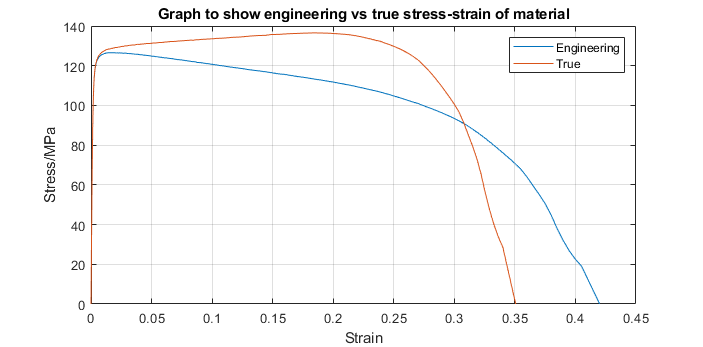
\includegraphics[width = \textwidth]{./img/engVsTrueStressStrain.png}
    \caption{Graph to show engineering vs true stress-strain response of material.}
    \label{engVsTrueStressStrainCurve}
\end{figure}
\subsection{Necking point/UTS}
To find the necking point, we need to find the ultimate tensile strength of our material, which can be found by indexing the largest stress value in our data.

Ultimate tensile strength (engineering):
\begin{gather}
    \sigma_{e,uts} = \SI{126.52}{\mega\pascal} \textrm{ at } \varepsilon = \SI{0.019}{}
\end{gather}
Ultimate tensile strength (true):
\begin{gather}
    \sigma_{t,uts} = \SI{136.51}{\mega\pascal} \textrm{ at } \varepsilon = \SI{0.186}{}
\end{gather}
We take the value from our true stress-strain curve as this accurately represents the stress-strain of our material until necking occurs.
\subsection{Effective stress-strain}
The effective stress-strain allows us to model the true undamaged stress-strain of the material. This is useful as ABAQUS requires this to model the behaviour of our material. This can be calculated by assuming a perfectly plastic response after the onset of necking:
\begin{gather}
    \widetilde{\sigma}_t = \begin{cases}
        \sigma_t & \textrm{for } \varepsilon_n \leq \varepsilon_{n,uts}\\
        \sigma_{n,uts}\left(1 + \varepsilon_n\right) & \textrm{for } \varepsilon_n > \varepsilon_{n,uts}
    \end{cases}\\
    \widetilde{\varepsilon}_t = \varepsilon_t
\end{gather}
A plot of the effective stress-strain curve is shown below.
\begin{figure}[H]
    \centering
    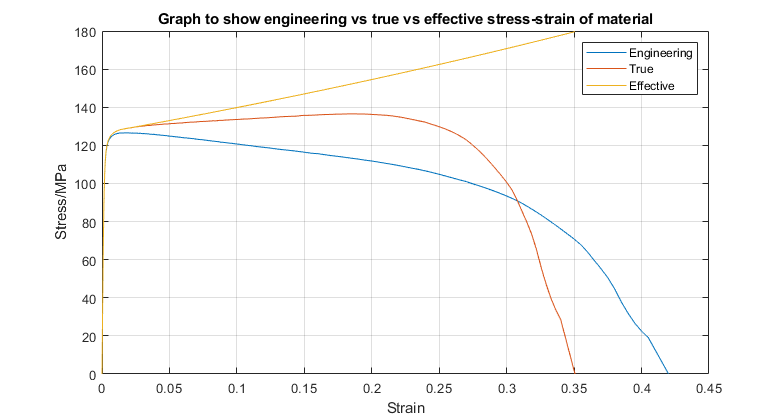
\includegraphics[width = \textwidth]{./img/engVsTrueVsEffectiveStressStrain.png}
    \caption{Graph to show engineering vs true vs effective stress-strain response of material.}
    \label{engVsTrueVsEffectiveStressStrainCurve}
\end{figure}
\subsection{Damage parameter}
The damage of the material is a measure of the area of voids in a material. The effective true stress can be written in terms of the damage variable:
\begin{align}
    \widetilde{\sigma}_t = \frac{F}{A-A_D} = \frac{F}{A\left(1 - \frac{A_D}{A}\right)} = \frac{\sigma_t}{1 - D}
\end{align}
Rewriting Hooke's Law:
\begin{gather}
    \widetilde{\sigma}_t = E \varepsilon_t \rightarrow \sigma_t = E\left(1-D\right)\varepsilon_t
\end{gather}
ABAQUS requires that damage evolution be inputted as a function fo the equivalent plastic displacement after necking, as strains are mesh dependent.
\begin{gather}
    \overline{u}_{pl} = L*\left(\overline{\varepsilon}^{pl}_t - \overline{\varepsilon}^{pl}_{t,uts}\right)
\end{gather}
where $L$ is the element size, $\overline{\varepsilon}^{pl}_t$ is the equivalent plastic strain and $\overline{\varepsilon}^{pl}_{t,uts}$ is the equivalent true plastic strain at the onset of necking. We also can see from the graph, that our damage parameter can easily be calculated as the difference between the damaged and undamaged stress-strain curves represents $D\widetilde{\sigma}_t$.
\subsection{Failure point}
As can be seen from the curves above, our failure point occurs at the strain where stress drops to 0. The engineering stress-strain is:
\begin{gather}
    \sigma_{n,f} = 0\\
    \varepsilon_{n,f} = 0.42
\end{gather}
True stress-strain:
\begin{gather}
    \sigma_{t,f} = 0\\
    \varepsilon_{t,f} = 0.3507
\end{gather}
\section{Description of FEM setup}
\subsection{Boundary and loading conditions}
The test sample was sketched and modelled in ABAQUS.
\begin{figure}[H]
    \centering
    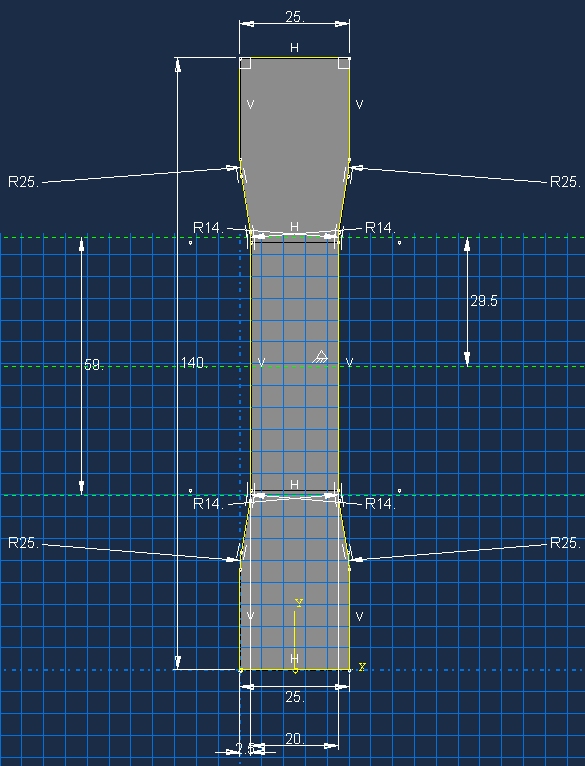
\includegraphics[width = 0.7\textwidth]{./img/Sketch1.png}
    \caption{Sketch of test sample in ABAQUS.}
    \label{sampleSketch}
\end{figure} 
The following boundary and loading conditions were applied:
\begin{itemize}
    \item Bottom fixed in U1, U2, UR3.
    \item Top displaced in U2 10 units upwards and fixed in U1 and UR3.
\end{itemize}
\subsection{Element type and justification}
Since we are looking at a relatively thin plate undergoing stresses in the $x$- and $y$- directions, we can model the plate in a 2D configuration with thickness \SI{1.5}{\milli\m}. We can assume here that through thickness stresses are zero and the in-plane stresses are constant through thickness in the component. We can make this assumption due to the relatively small thickness of the plate in comparison to its other dimensions. Hence, we can choose to focus on plane stress for our simulation.
\begin{gather}
    \sigma_z = \sigma_{zx} = \sigma_{zy} = \varepsilon_{zx} = \varepsilon_{zy} = 0
\end{gather}
A quad element type was used to mesh the sample. This is because our sample requires a high degree of precision in the test region. Quad elements can accurately break down the geometry of the sample in the analysis, as it has a rectangular section. Using quad elements will also allow us to have a small aspect ratio and create a structured mesh. 
\subsection{Material models employed}
A new material (labeled `alu') was created in ABAQUS with the following properties:
\begin{itemize}
    \item Elastic
    \begin{itemize}
        \item Young's modulus: \SI{67114.97}{\giga\pascal} (MATLAB variable \texttt{`YM'})
        \item Poission's ratio: 0.3 (given)
    \end{itemize}
    \item Plastic
    \begin{itemize}
        \item Yield stress and plastic strain: tabular data (MATLAB variable \texttt{`plasticYield'})
    \end{itemize}
    \item Ductile damage
    \begin{itemize}
        \item Fracture strain: 0.015 (MATLAB variable \texttt{`equivTrueUTSPlasticStrain'})
        \item Stress triaxiality: 0.333 (given)
        \item Strain rate: 0
    \end{itemize}
    \item Damage evolution: 
    \begin{itemize}
        \item type - displacement, softening - linear, displacement at failure: 0.3212 (MATLAB tabular data \texttt{`equivPlasticDisp'}). Used for testing mesh convergence
        \item type - displacement, softening - tabular, damage variables calculated in MATLAB (\texttt{`damage'} variable). Used to test properties of material failure.
    \end{itemize}
\end{itemize}
Since we need to input true plastic strain values into ABAQUS, we need to calculate it by using the following formula:
\begin{gather}
    \varepsilon^{pl}_t = \varepsilon_t - \varepsilon_{t,yield}
\end{gather}
We can also calculate the aforementioned fracture strain (\texttt{`equivTrueUTSPlasticStrain'}:
\begin{gather}
    \varepsilon^{pl}_{t,UTS} = 0.015 
\end{gather}
The calculations were made in MATLAB and a plot is shown below. 
\begin{figure}[H]
    \centering
    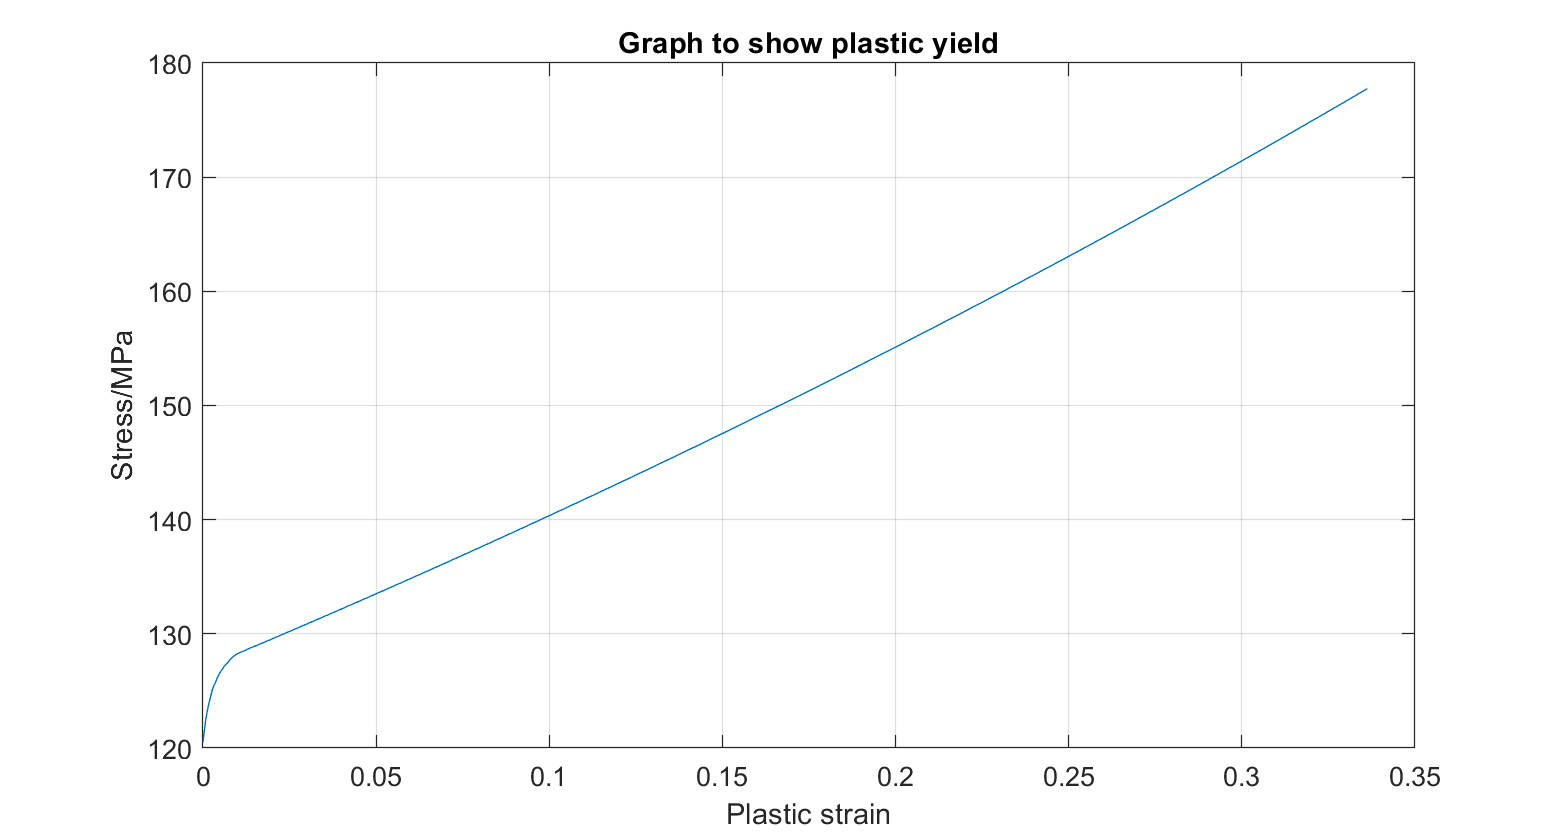
\includegraphics[width = 0.9\textwidth]{./img/plasticYield.png}
    \caption{Graph to show plastic yield.}
\end{figure}
We also need to generate the tabular data for our damage parameter, which can be found by finding the difference in value between our damaged and undamaged stress-strain curves. Calculation was done in MATLAB and a plot is shown below.
\begin{figure}[H]
    \centering
    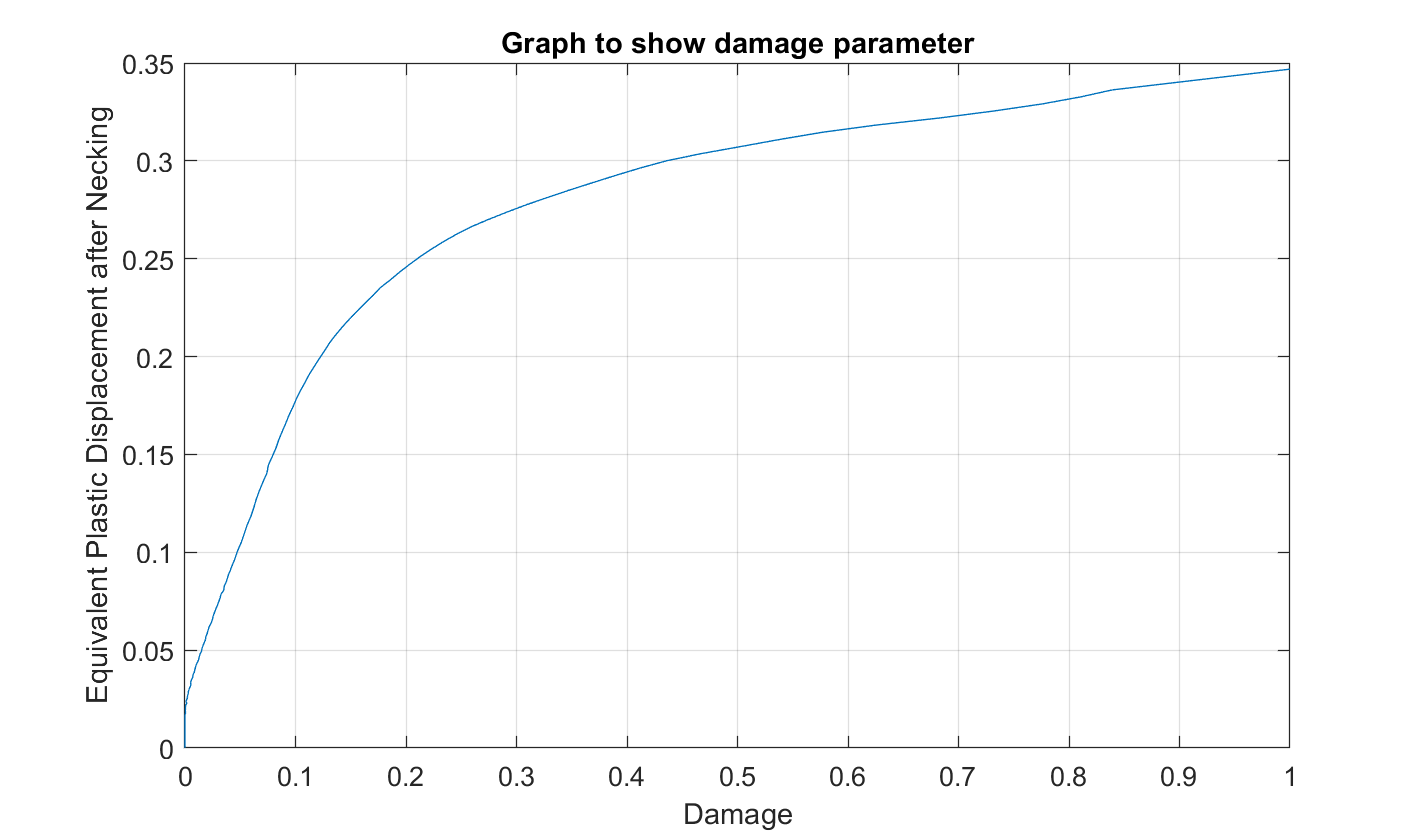
\includegraphics[width = 0.9\textwidth]{./img/damage.png}
    \caption{Graph to show damage parameter.}
\end{figure}
\subsection{Mesh configuration and convergence}
As our model involves variables which are sensitive to mesh size, choosing an appropriate mesh size is important to ensure accurate results. The main parameters to focus on are the parameter of interest (stress) and the computational run time. The table below shows how varying the mesh size affects our simulation results. A linear damage model was used to simplify the results. 
\begin{table}[H]
    \resizebox*{\textwidth}{!}{
    \begin{tabular}{@{}llllllll@{}}
    \toprule
    Mesh size & no. of elements & Run time/s & Type of break    & LE22 max & S22 max/MPa & Mises max/MPa & error/\% \\ \midrule
    4         & 216             & 3.5        & Horizontal crack & 0.3775   & 128.877     & 128.862       & 0.52     \\ 
    2         & 770             & 5.4        & Cup and cone     & 0.3339   & 129.352     & 128.815       & 0.08     \\ 
    1         & 3080            & 33.8       & Cup and cone     & 0.3507   & 129.502     & 128.909       & 0.20     \\ 
    0.8       & 4752            & 47.5       & Cup and cone     & 0.3478   & 129.121     & 128.908       & 0.10     \\ 
    0.5       & 12364           & 99.9       & Cup and cone     & 0.3443   & 129.448     & 128.902       & 0.15     \\
    0.3       & 35100           & 397.3      & Cup and cone     & 0.3406   & 129.773     & 128.916       & 0.38     \\
    0.2       & 78030           & 1013.1     & Cup and cone     & 0.3674   & 129.248     & 128.908       & 0        \\ \bottomrule
    \end{tabular}
    }
\end{table}
A mesh size of 0.8 was selected as it offers accurate results for a relatively low computational time. 
\section{Post-Processing and examination of results from FEA}
The simulation was run and the results extracted. Using the timeline view, we can see that elements are deleted from the centre of the specimen and gradually propagates to a crack and split of the specimen into two. The logarithmic strain in LE22 and true stress in S22 was outputted from ABAQUS and plotted below.
\begin{figure}[H]
    \centering
    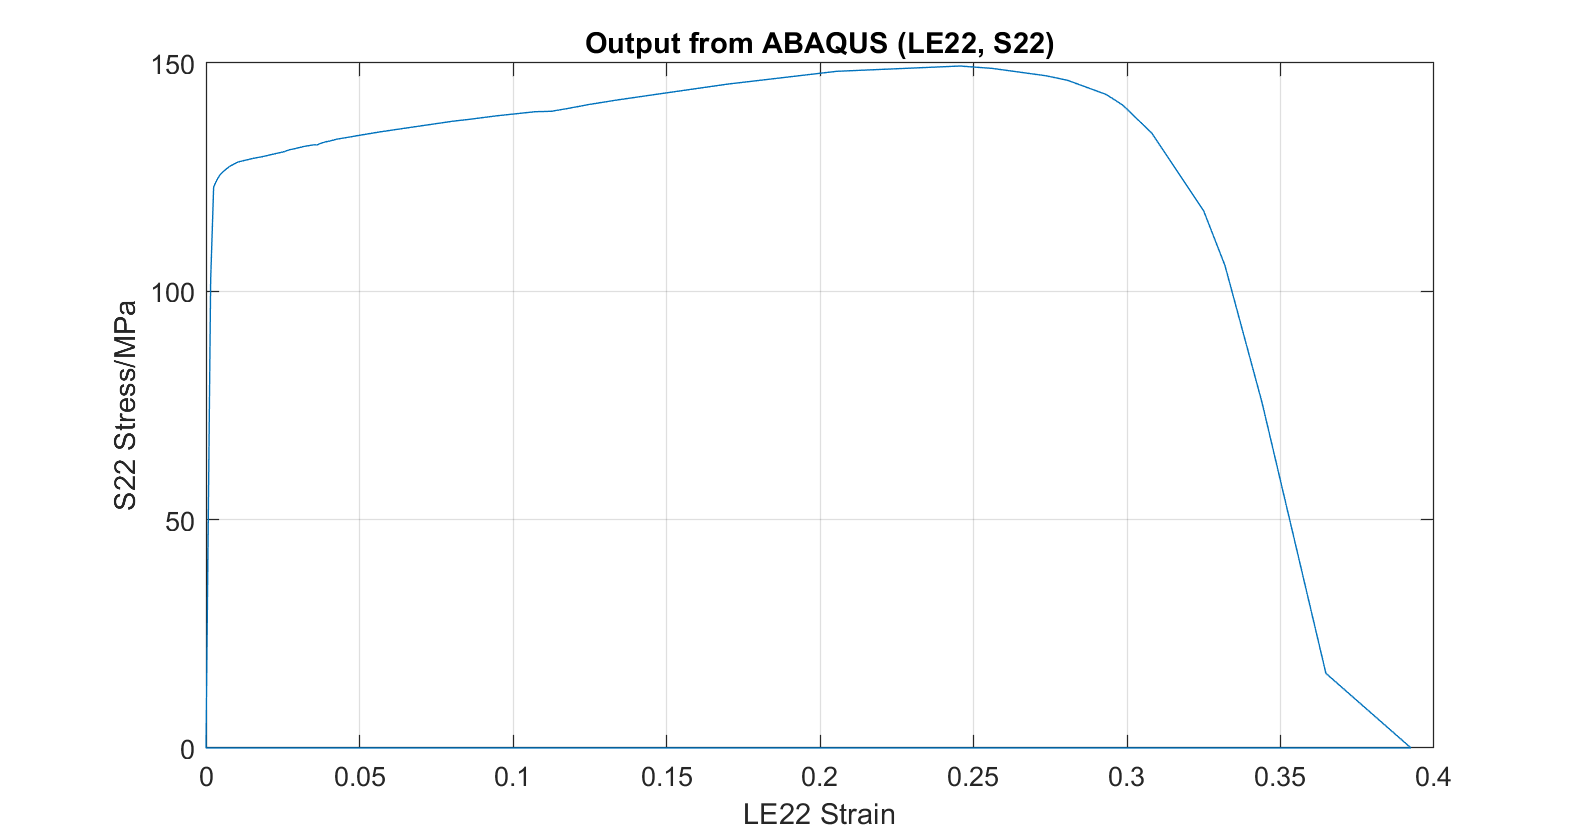
\includegraphics[width = 0.8\textwidth]{./img/s22Strain.png}
    \caption{Field output from ABAQUS (LE22, S22)}
\end{figure}
LE22 is a valid field output as it takes into account the deformation per increment which incorporates the strain path. This means that it accurately represents our longitudinal strain. 
\subsection{Elastic region}
\begin{figure}[H]
    \centering
    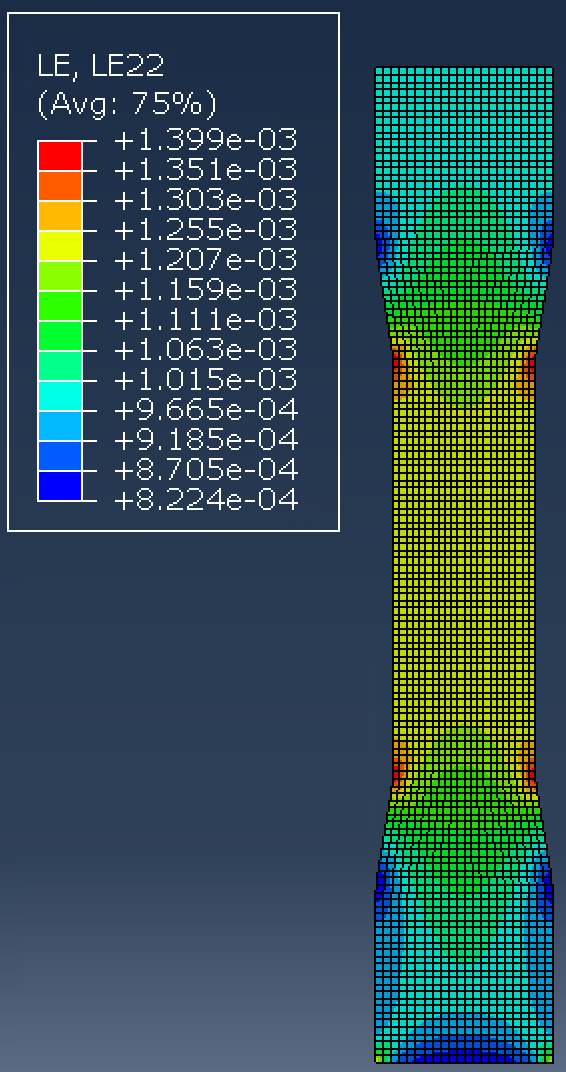
\includegraphics[width = 0.3\textwidth]{./img/elastic.png}
    \caption{Field output of elastic state}
\end{figure}
\subsection{Onset of plasticity}
\begin{figure}[H]
    \centering
    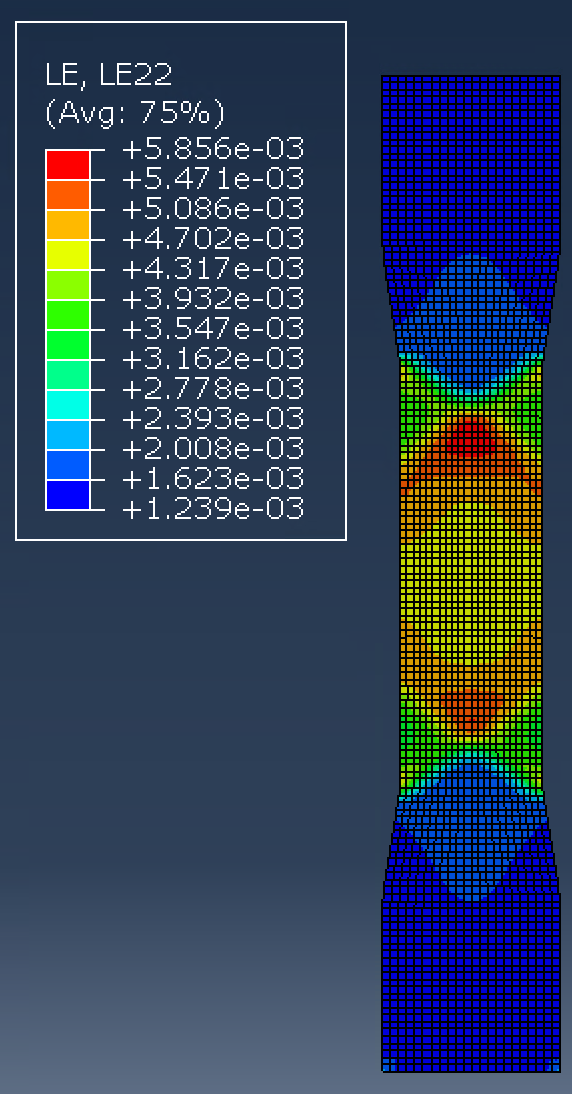
\includegraphics[width = 0.3\textwidth]{./img/onset1.png}
    \caption{Field output from before onset of plasticity}
\end{figure}
\begin{figure}[H]
    \centering
    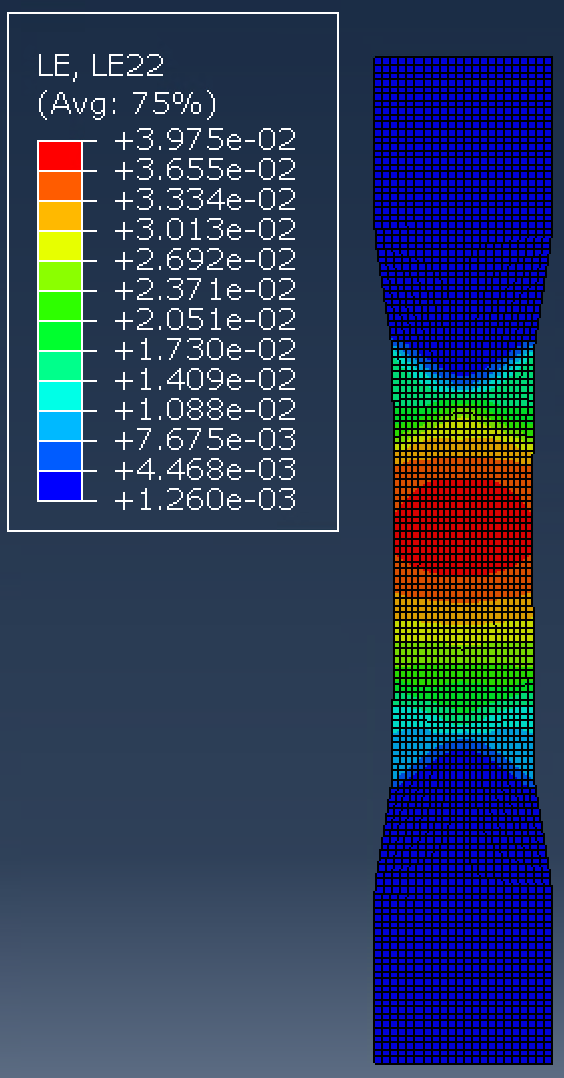
\includegraphics[width = 0.3\textwidth]{./img/onset2.png}
    \caption{Field output from after onset of plasticity}
\end{figure}
\subsection{Plastic hardening}
\begin{figure}[H]
    \centering
    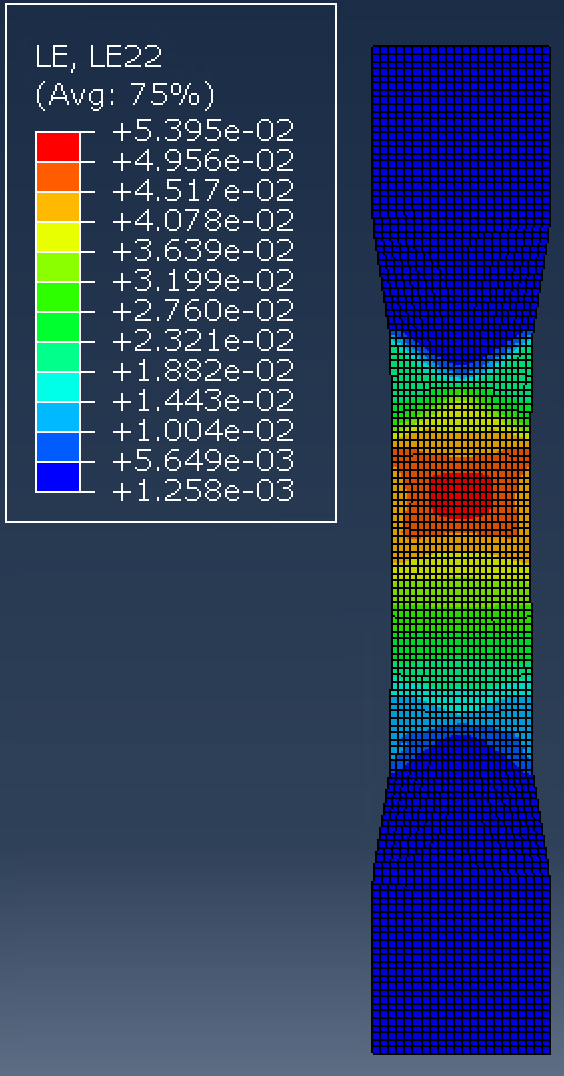
\includegraphics[width = 0.3\textwidth]{./img/plasticHardening.png}
    \caption{Field output of plastic hardening state}
\end{figure}
\subsection{Onset of necking}
\begin{figure}[H]
    \centering
    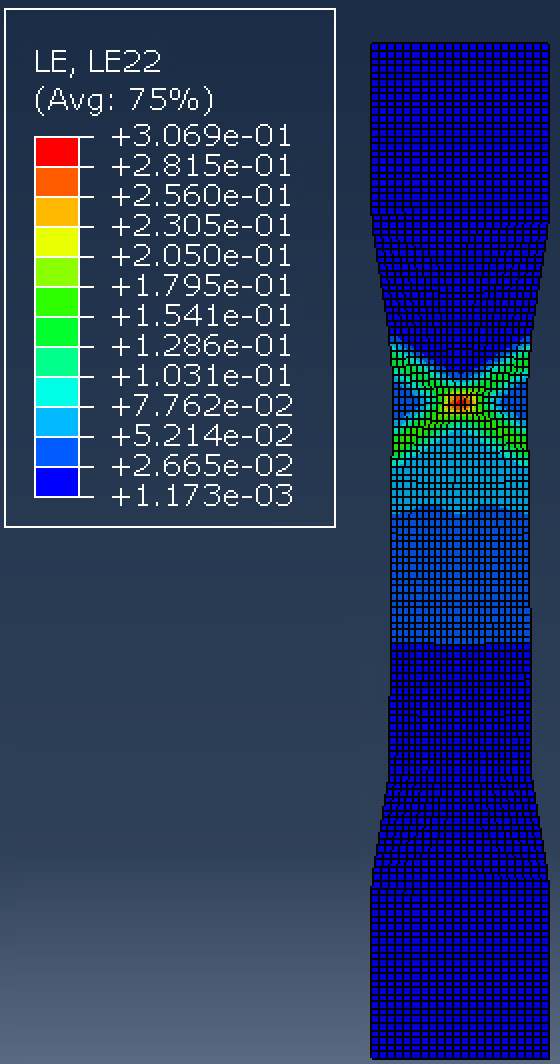
\includegraphics[width = 0.3\textwidth]{./img/necking.png}
    \caption{Field output of necking state}
\end{figure}
\subsection{Softening and formation of voids}
\begin{figure}[H]
    \centering
    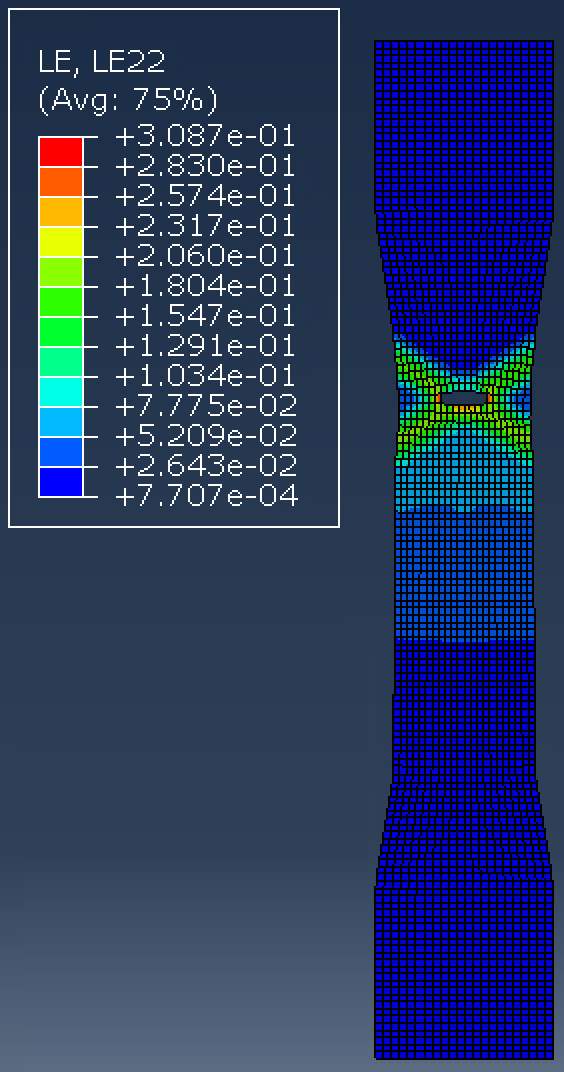
\includegraphics[width = 0.3\textwidth]{./img/softening.png}
    \caption{Field output from softening state}
\end{figure}
\begin{figure}[H]
    \centering
    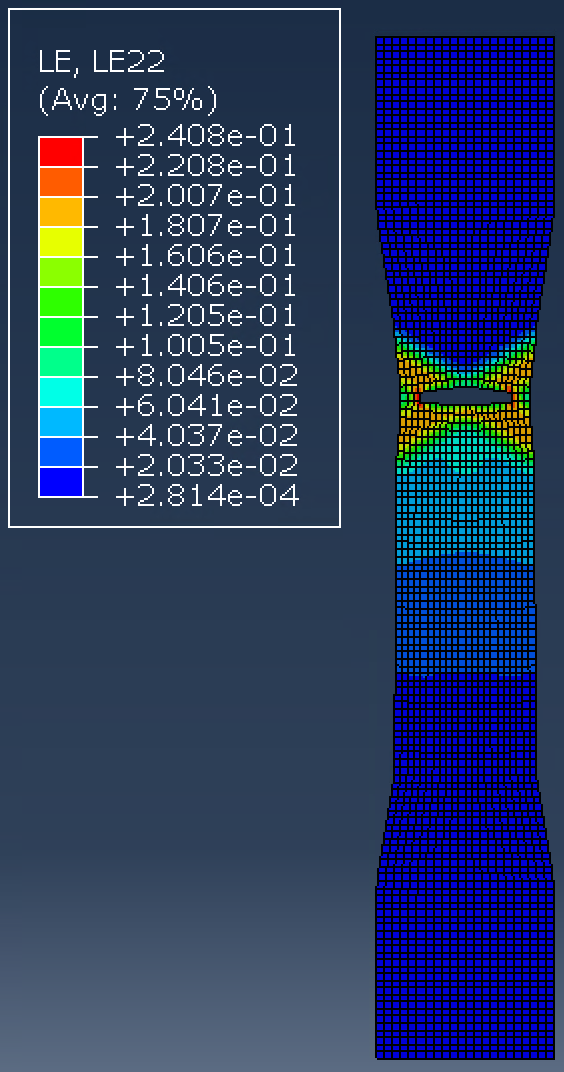
\includegraphics[width = 0.3\textwidth]{./img/softening2.png}
    \caption{Field output from softening state (crack propagation)}
\end{figure}
\begin{figure}[H]
    \centering
    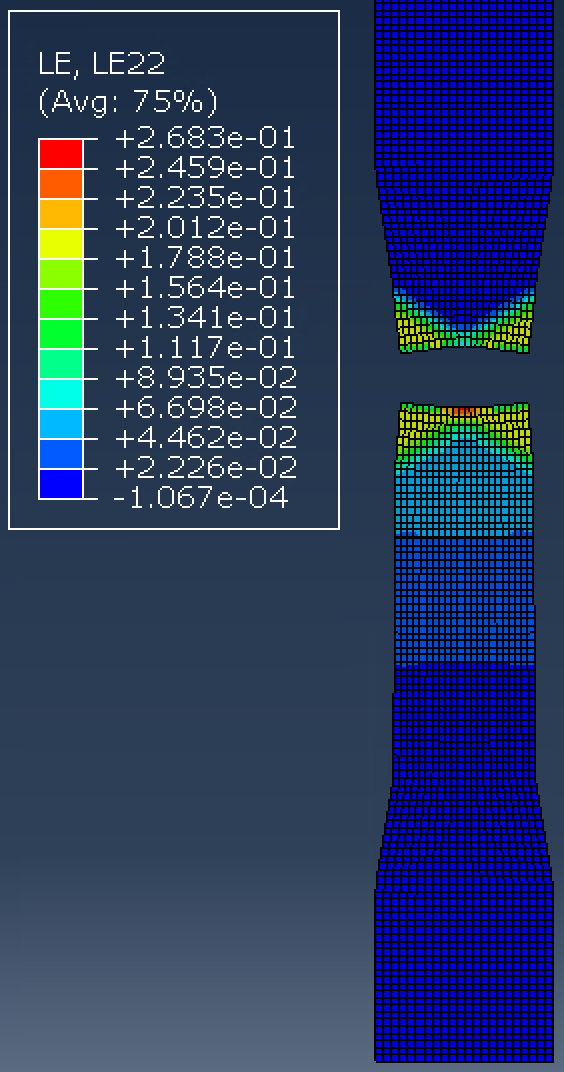
\includegraphics[width = 0.3\textwidth]{./img/softening3.png}
    \caption{Field output from softening state (failure)}
\end{figure}
\section{Discussion}
\subsection{Analytical vs FEA data}
\begin{figure}[H]
    \centering
    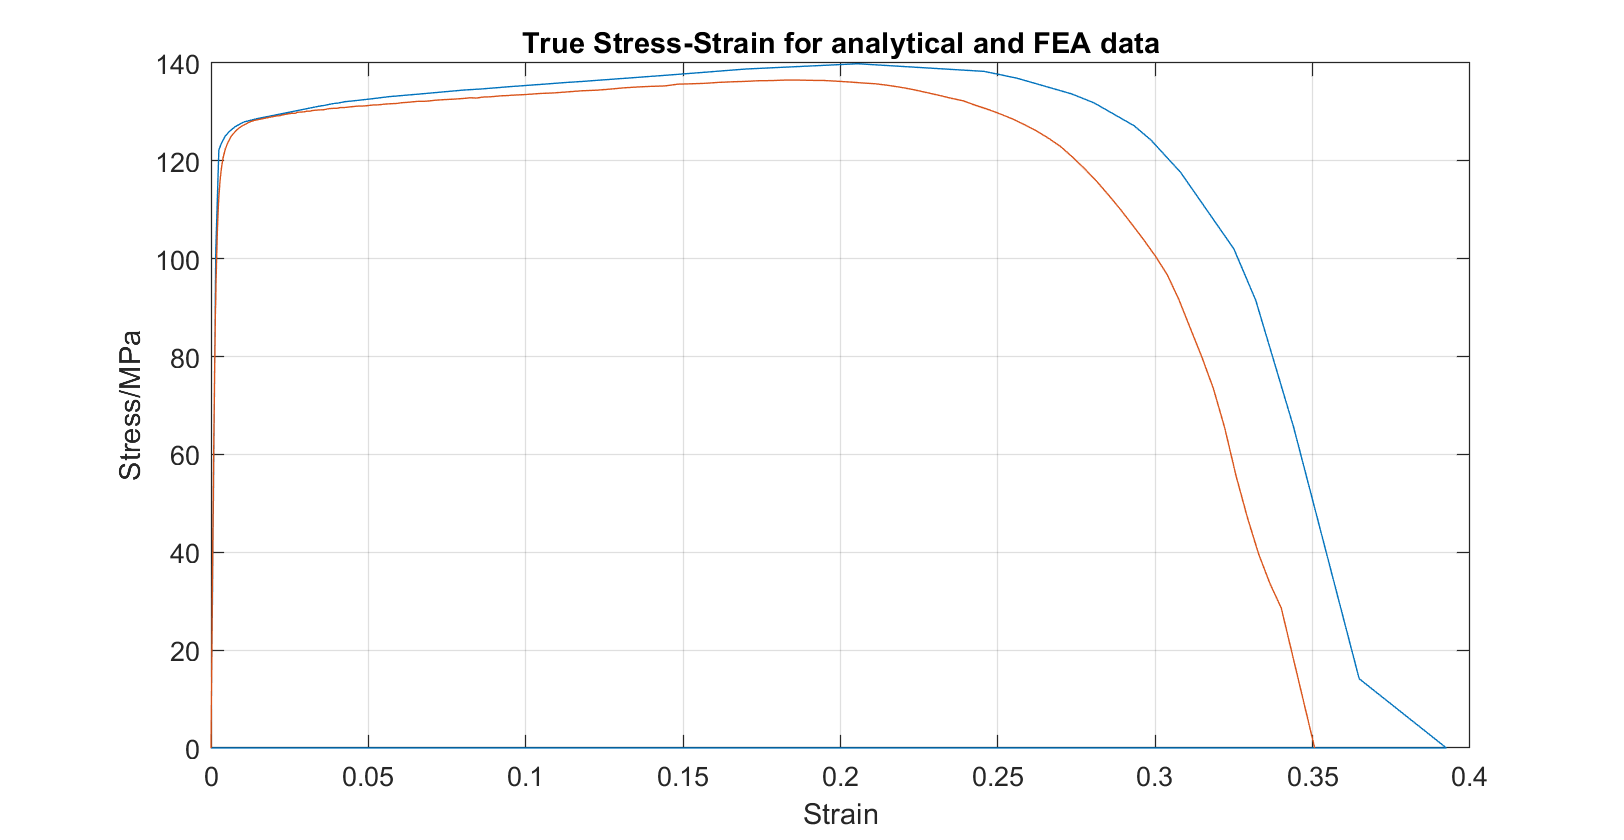
\includegraphics[width = \textwidth]{./img/comparisonData.png}
    \caption{Graph to show analytical vs FEA data. Orange analytical, blue FEA.}
\end{figure}
The Mises stress was pulled from ABAQUS and plotted against the LE22 strain. This is because ABAQUS uses Mises stress to define the plastic yielding properties \cite{b3}. We can see that the curves follow quite closely initially but after the onset of necking our results differ. This could be due to the damage model used in ABAQUS. We find that the ABAQUS model has more true stress for the same true strain compared to the analytical data.
\subsection{Material model}
We find that FEA accurately portrays the phases from elastic to plastic hardening reasonably well. This tells us that our initial calculations for Young's Modulus, yield point and UTS were correct and accurate. This also shows that our assumptions about yield stress were correct (using a 0.2\% offset). 

However, towards the hardening and softening phases of our FEA model, we see our results start to differ. This may be due to the damage model used, which incorporates a damage function derived from the effective and true stress-strain curves. We have also made assumptions about our sample in our analysis. In FEA, our material will be `perfect' in the sense that it will not have microvoids and stress concentrators. These naturally serve to decrease the stress tolerable by a real life sample. Hence, this could be why we see FEA giving us higher values for a given strain. 
\subsection{Failure initiation and propagation}
We see that our crack forms towards the top of the thin part of the sample. First, we see that our material starts to thin (necking) and the shear lines are clearly visible and the first voids form. We then see that our crack propagates outwards and horizontally. However, this should not be the case for ductile materials like aluminium. We should see a \SI{45}{\degree} crack propagation from the initial void. This is because shear stress is the dominant force and this occurs at \SI{45}{\degree}. The crack propagates from the centre and progresses outwards, which is accurate as the void in the centre would act as a stress concentrator and fractures would form from there. 
\newpage
\begin{thebibliography}{00}
    \bibitem{b1} Illinois Tool Works, (2022) `Offset Yield Strength' \url{https://www.instron.com/en-gb/our-company/library/glossary/o/offset-yield-strength} Accessed: 01/03/22
    \bibitem{b2} ASTM, (2022) `Standard Test Methods for Tension Testing of Metallic Materials' \url{https://www.astm.org/e0008_e0008m-21.html} Accessed: 01/03/22
    \bibitem{b3} ABAQUS Documentation, (2022) `Post Processing Plasticity data ABAQUS' \url{https://abaqus-docs.mit.edu/2017/English/SIMACAEGSARefMap/simagsa-c-matpostprocess2.htm} Accessed: 02/03/22
\end{thebibliography}
\end{document}